\chapter{Современные системы управления}

Современные технологические процессы повышают требования для качества управления. Исследователи применяют для решения задач в данной области множество методов, в том числе искусственные нейронные сети, имеющие высокий потенциал в этой области. Однако они не обеспечивают значимых преимуществ перед классическими подходами и требуют улучшения.
В данной главе рассматриваются современные технологии и методы, применяемые в системах управления технологическими процессами, оценивается их эффективность и недостатки. Определены исходные данные для анализа и параметры качества. Выполнена постановка задачи исследования.

\section{ПИД-регуляторы}

ПИД-регуляторы доказали свою эффективность в управлении разнообразными процессами. Их использование не требует знания точной модели процесса, поэтому они эффективны в управлении промышленными и технологическими процессами, математические модели которых достаточно сложно определить. ПИД-регуляторы строятся на основе классической теории управления и просты для понимания и реализации (рис. \ref{fig:PID_controller_scheme}).

\begin{figure}[H]
    \centering
    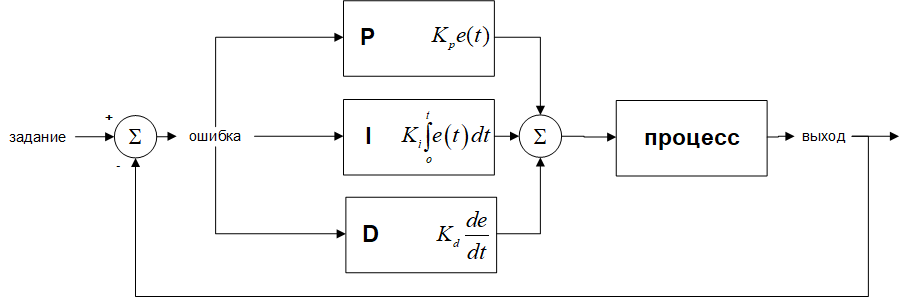
\includegraphics[width=\textwidth]{images/chapter1/Структурная схема ПИД-регулятора.png}
    \caption{Структурная схема ПИД-регулятора}
    \label{fig:PID_controller_scheme}
\end{figure}

\subsection{Описание ПИД-регуляторов}

Назначение ПИД-регулятора – в поддержании заданного значения $x_0$ некоторой величины $x$ с помощью изменения другой величины $u$. Значение $x_0$ называется заданием, а разность $e=(x_0-x)$ – невязкой или рассогласованием. Выходной сигнал контроллера $u$ определяется тремя слагаемыми:

\begin{equation}
    \label{eq_PID}
    u(t) = P + I + D = K_p e(t) + K_i \int_{0}^{t} e(t) dt + K_d \frac{de}{dt}
\end{equation}

где $K_p, K_i, K_d$ – коэффициенты усиления пропорциональной, интегральной и дифференциальной составляющих контроллера, соответственно.
Большинство методов настройки ПИД-регулятора используют несколько иную формулу для выходного сигнала, в которой на пропорциональный коэффициент усиления умножены также интегральная и дифференциальная составляющие:

\begin{equation}
    u(t) = K_p \left( e(t) + \frac{1}{T_i} \int_{o}^{t} e(\tau) d \tau +T_d \frac{de}{dt}\right).
\end{equation}

\textbf{Пропорциональная составляющая} – $K_p$ – вырабатывает выходной сигнал, который стабилизирует отклонение регулируемой величины. Выходной сигнал пропорциональной составляющей тем больше, чем сильнее регулируемая величина отклоняется от задания. Если входной сигнал равен заданию, то выходной равен нулю.

При использовании пропорционального контроллера значение регулируемой величины никогда не стабилизируется на заданном значении. Существует так называемая статическая ошибка, которая равна такому отклонению регулируемой величины, которое обеспечивает выходной сигнал, стабилизирующий выходную величину именно на этом значении. Например, в контроллере температуры выходной сигнал (мощность нагревателя) постепенно уменьшается при приближении температуры к заданию, и система стабилизируется при мощности равной тепловым потерям. Температура не может достичь задания, так как в этом случае мощность нагревателя станет равна нулю, и он начнет остывать.

Чем больше коэффициент пропорциональности между входным и выходным сигналом (коэффициент усиления), тем меньше статическая ошибка, однако при слишком большом коэффициенте усиления могут начаться автоколебания, а при дальнейшем увеличении коэффициента система может потерять устойчивость.

Для устранения статической ошибки используют \textbf{интегральную составляющую} – $K_i$. Она позволяет регулятору «учиться» на предыдущем опыте. Если система не испытывает внешних возмущений, то через некоторое время регулируемая величина стабилизируется на заданном значении, сигнал пропорциональной составляющей будет равен нулю, а выходной сигнал будет полностью обеспечивать интегральная составляющая.

\textbf{Дифференциальная составляющая} – $K_d$ – противодействует предполагаемым отклонениям регулируемой величины, которые могут произойти в будущем. Эти отклонения могут быть вызваны внешними возмущениями или запаздыванием воздействия регулятора на систему. Чем быстрее регулируемая величина отклоняется от задания, тем сильнее противодействие, создаваемое дифференциальной составляющей.

\subsection{Достоинства и недостатки ПИД-регуляторов}

Установление связей между параметрами и управление действиями системы может осуществляться инженерами-практиками и операторами.
Кроме того, за последние десятилетия разработано несколько методов настройки ПИД-регуляторов.

Однако, наряду с вышеуказанными достоинствами, ПИД-регуляторы имеют и ряд недостатков. Так, если рабочая точка процесса изменяется из-за возмущений, параметры контроллера требуется перенастраивать вручную, чтобы получить новую оптимальную настройку. Настройка должна осуществляться опытным оператором. Для систем с взаимодействующими контурами это процедура может быть сложной и занимать много времени. Кроме того, для процессов с переменными параметрами, временными задержками, существенными нелинейностями и значительными помехами использование ПИД-регуляторов может не обеспечить оптимальных характеристик.

Методы настройки ПИД-регуляторов также имеют ряд недостатков.
Одна из идей повышения эффективности ПИД-регуляторов заключается в управлении с самонастройкой, в котором параметры контроллера настраивались бы в оперативном режиме.

\subsection{Дискретная реализации ПИД-регулятора}

Идеализированное уравнение ПИД-регулятора (\ref{eq_PID}) является непрерывным, т. е. использует непрерывное время. При построении регулятора на базе компьютера входные и выходные переменные регулятора необходимо квантовать по времени с некоторым шагом $T_0$, и преобразовать в цифровую форму с помощью аналого-цифровых и цифро-аналоговых преобразователей. При этом уравнение ПИД-регулятора должно быть преобразовано в разностное с помощью замены производных конечной разностью, а интеграла – конечной суммой. В зависимости от выбранного метода перехода от непрерывных операторов к их дискретным аналогам возникает несколько различных уравнений, описывающих дискретные ПИД-регуляторы. При использовании метода прямоугольников для замены интеграла конечной суммой получим \cite{PID_NIL_AP}:


\begin{equation}
    \label{eq_discrete_PID}
    u(k) = K\left[ e(k) + \frac{T_0}{T} \sum_{i = 0}^{k} {e(i - 1)} + \frac{T_D}{T_0} (e(k) - e(k - 1))\right],
\end{equation}

где $k = 0, 1, \ldots\frac{t}{T_0}$ - порядковый номер отсчета дискретного времени.

Недостатком такого представления уравнения регулятора является необходимость помнить значения отклонений $e(k)$ для всех моментов времени от начала процесса регулирования.

Этот недостаток можно устранить, если для вычисления текущего значения управляющей переменной $u(k)$ использовать ее предыдущее значение $u(k-1)$ и поправочный член. Для получения такого рекуррентного алгоритма достаточно вычесть из уравнения (\ref{eq_discrete_PID}) следующее уравнение \cite{PID_NIL_AP}:

\begin{displaymath}
    u\left(k-1\right)=K\left[e\left(k-1\right)+\frac{T_0}{T}\sum_{i=0}^{k-1}{e(i-1)}+\frac{T_D}{T_0}(e\left(k-1\right)-e(k-2))\right].
\end{displaymath}

В результате получим [6]:

\begin{equation}
    u\left(k\right)-u\left(k-1\right)=q_0e\left(k\right)+q_1e\left(k-1\right)+q_2e\left(k-2\right),
\end{equation}

Где

\begin{equation}
    q_0=\mathbf{K}\left(1+\frac{T_D}{T_0}\right),
\end{equation}

\begin{equation}
    q_1=-\mathbf{K}\left(1+2\frac{T_D}{T_0}-\frac{T_0}{T_D}\right),
\end{equation}

\begin{equation}
    q_2=\mathbf{K}\frac{T_D}{T_0}.
\end{equation}

Таким образом, для вычисления текущего значения управляющего воздействия $u(k)$ на объект управления достаточно хранить в памяти только величины $u\left(k-1\right)$, $e\left(k\right)$, $e\left(k-1\right)$, $e(k-2)$, то есть величины

\begin{equation}
    u\left(k\right)=u\left(k-1\right)+\Delta u(k),
\end{equation}

\begin{equation}
    \Delta u\left(k\right)=q_0e\left(k\right)+q_1e\left(k-1\right)+q_2e\left(k-2\right).
\end{equation}

Итак, алгоритм работы ПИД-регулятора может быть представлен в следующем виде [3]:

\begin{equation}
    u\left(k\right)=u\left(k-1\right)+\Delta u(k),
\end{equation}

\begin{equation}
    \Delta u\left(k\right)=q_0e\left(k\right)+q_1e\left(k-1\right)+q_2e\left(k-2\right),
\end{equation}

\begin{equation}
    q_0=\mathbf{K}\left(1+\frac{T_D}{T_0}\right), q_1=-\mathbf{K}\left(1+2\frac{T_D}{T_0}-\frac{T_0}{T_D}\right), q_2=\mathbf{K}\frac{T_D}{T_0}.
\end{equation}

При переходе от непрерывных операторов к дискретным возникает погрешность, величина которой пропорциональна остаточному члену ряда Тейлора функции $e\left(t\right)$. Поэтому полученные дискретные уравнения можно считать эквивалентными непрерывным только при условии, что $e\left(t\right)$ изменяется слабо в пределах такта квантования. Однако с помощью аппарата z-преобразования можно показать, что основные свойства ПИД-регулятора сохраняются и при больших шагах квантования, если параметры регулятор $q_0$, $q_1$, $q_2$ выбирать не на основании параметров его непрерывного аналога, а независимо от них, методами параметрической оптимизации, выбрав необходимый критерий качества оптимизации исходя из цели регулирования. Такт квантования выбирают аналогично \cite{PID_NIL_AP}.